\section{Evaluation}
\label{sec:results}

\begin{table*}[t]
% \setlength{\tabcolsep}{3pt}
\centering
\scriptsize
\begin{tabular}{|l|c|l|r|r||r|r|r|r||r|r|r|r|c|}

\hline
\multicolumn{1}{|c|}{\textbf{API}} &
\multicolumn{1}{c|}{\textbf{BugID}} &
\multicolumn{1}{c|}{\textbf{Priority}} &
\multicolumn{1}{c|}{\textbf{$\mathcal{N}_{CG}$}} &
\multicolumn{1}{c||}{\textbf{$\mathcal{N}_{Unit}$}} &
%\multicolumn{1}{c|}{\textbf{$PPI$}} &
\multicolumn{1}{c|}{\textbf{$\mathcal{S}_{U}$}} &
\multicolumn{1}{c|}{\textbf{$\mathcal{F}_{U}$}} &
\multicolumn{1}{c|}{\textbf{$\mathcal{S}_{P}$}} &
\multicolumn{1}{c||}{\textbf{$\mathcal{F}_{P}$}} &
\multicolumn{1}{c|}{\textbf{$PPI$}} &
\multicolumn{1}{c|}{\textbf{$FCI$}} &
\multicolumn{1}{c|}{\textbf{$\mathcal{IC}_{NO}$}} & %instrumentation with
%optimization
\multicolumn{1}{c|}{\textbf{$\mathcal{IC}_{WO}$}} & %instrumentation without
% optimization
\multicolumn{1}{c|}{\textbf{$\mathcal{RS}_{CE}$}}  % cascaded exception
%new added col
\\

\hline
\code{Aries} & \cite{ARIES1204} & Major &$3.5K$  & $1.02$ & 
$18$ & $2$ & $20$ & $0$ & $0.83$ & $0$ & $42$ & $5$ & $\checkmark$ \\

\code{Commons CLI1.x} & \cite{CLI193} & Critical & $3.2K$ & $53$ & 
$14$ & $2$ & $16$ & $0$ & $0.74$ &$0$ & $19$& $19$ & $\checkmark$ \\

\code{Commons CLI2.x} & \cite{CLI46} & Major & $3.2K$ & $21$ & 
$13$ & $3$ & $16$ & $3/1$ & $0.62$ &$1$ & $13$ &$2$ & $\times$\\

\code{Commons Compress} & \cite{COMPRESS26} & Blocker & $4.0K$ & $134$ & 
$32$ & $1$ & $33$ & $0$ & $0.74$ &$0$ & $46$& $4$ &$\checkmark$ \\

\code{Commons IO} & \cite{IO179} & Major & $3.3K$ & $125$ & 
$27$ & $1$ & $28$ & $0$ & $0.77$ &$0$ & $76$ & $1$ & $\checkmark$ \\

\code{Commons Lang} & \cite{LANG457} & Major & $5.1K$ & $240$ & 
$16$ & $2$ & $18$ & $0$ & $0.59$ &$0$ & $168$& $8$ & $\checkmark$ \\

\code{Commons Math} & \cite{MATH198} & Major & $3.4K$ & $300$ & 
$19$ & $2$ & $21$ & $2/0$ & $0.89$ &$1$ & $36$ &$2$ & $\checkmark$ \\
 
\code{Commons Net} & \cite{NET442} & Major & $3.3K$ & $14$ & 
$22$ & $1$ & $23$ & $0$ & $0.84$ &$0$ & $6$ & $1$ & $\checkmark$ \\

\code{Commons VFS} & \cite{VFS338} & Major &$4.5K$ & $37$ & 
$18$ & $1$ & $19$ & $0$ & $0.65$ &$0$ & $20$ & $2$ & $\checkmark$ \\

\code{Derby} & \cite{DERBY4748} & Major & $4.4K$ & $40$ & 
$30$ & $2$ & $22$ & $0$ & $0.46$ &$0$ & $47$ & $6$ & $\checkmark$ \\

\code{Eclipse AJ Weaver} & \cite{EclipseBug432874} & Major & $20.6K$ & $50$ &
$17$ & $2$ & $17$ & $2$ & $0.98$ &$0$ & $4$ & $1$ & $\times$ \\

\code{Eclipse AJ} & \cite{EclipseBug333066} & Major & $25.0K$ &$39$ & 
$14$ & $2$ & $16$ & $0$ & $0.87$ &$0$ & $6$ & $1$ &$\checkmark$ \\

\code{FlexDK 3.4} &\cite{SDK14417} & Minor & $6.3K$ & $600$ & 
$13$ & $2$ & $15$ & $0$ & $0.74$ &$0$ & $207$ & $25$& $\checkmark$ \\

\code{Hama 0.2.0} &\cite{HAMA212}  & Critical & $3.7K$ & $35$ & 
$13$ & $1$ & $14$ & $0$ & $0.55$ &$0$ & $28$ & $5$ & $\checkmark$ \\

\code{HBase 0.92.0} &\cite{HBASE4481}  & Critical & $4.8K$ & $61$ & 
$24$ & $1$ & $25$ & $0$ & $0.83$ &$0$ & $13$ & $2$ & $\checkmark$ \\

\code{Hive} &\cite{HIVE6986} & Trivial &$4.4K$ & $23$ & 
$18$ & $1$ & $18$ & $1$ & $0.75$ &$0$ & $8$ & $1$ & $\checkmark$ \\

\code{HttpClient} &\cite{HTTPCLIENT150} & Major & $3.3K$ & $14$ & 
$20$ & $3$ & $23$ & $0$ & $0.89$ &$0$ & $6$& $1$ & $\checkmark$ \\

\code{jUDDI} & \cite{JUDDI292} & Major &$3.2K$ & $70$ & 
$28$ & $1$ & $29$ & $0$ & $0.85$ &$0$ & $10$ & $2$ & $ \checkmark$ \\

\code{Log4j} & \cite{ApacheLog4jBug} & Major & $3.2K$ & $17$ & 
$8$ & $3$ & $11$ & $0$ & $0.74$ & $0$ & $6$ &$1$ & $\checkmark$ \\

\code{MyFaces Core} & \cite{MYFACES416} & Major  & $4.5K$ & $50$ &
$11$ & $3$ & $14$  & $0$ & $0.83$ & $0$ & $4$& $2$ & $\checkmark$ \\

\code{Nutch} & \cite{NUTCH1547} & Major & $4.5K$ & $90$ & 
$8$ & $3$ & $11$ & $0$ & $0.68$ &$0$ & $8$ & $1$ & $\checkmark$ \\

\code{Ofbiz} & \cite{OFBIZ4237} & Minor & $4.4K$ & $28$ & 
$20$ & $3$ & $26$ & $3/0$ & $0.45$ &$1$ & $6$ &$1$ & $\checkmark$ \\

\code{PDFBox} & \cite{PDFBOX467} & Major &$4.4K$ & $23$ & 
$15$ & $3$ & $18$ & $0$ & $0.87$ &$0$ & $8$ & $1$ & $\checkmark$ \\

\code{Sling Eclipse IDE} & \cite{SLING3095} & Major & $4.5K$ & $58$ & 
$5$ & $1$ & $6$ & $0$ & $0.59$ & $0$ &$39$ & $6$ & $\checkmark$ \\

\code{SOAP} & \cite{SOAP130} & Major &$5.0K$ & $165$ & 
$18$ & $3$ & $21$ & $3/0$ & $0.84$ & $1$ & $32$ & $5$ & $\checkmark$ \\

\code{SOLR 1.2} & \cite{SOLR331} & Major & $11.0K$ & $200$ & 
$12$ & $2$ & $14$ & $0$ & $0.89$ & $0$ & $25$ & $4$ & $\checkmark$ \\

\code{Struts2} & \cite{WW650} & Major & $16.0K$ & $80$ & 
$11$ & $2$ & $13$ & $0$ & $0.76$ &$0$ & $25$ & $2$ & $\checkmark$ \\

\code{Tapestry 5} & \cite{TAP51770} & Major & $6.2K$  & $71$ & 
$17$ & $3$ & $20$ & $0$ & $0.70$ &$0$ & $31$ &$5$ & $\checkmark$ \\

\code{Wicket} & \cite{WICKET4387} & Major & $70.0K$ & $68$ & 
$20$ & $3$ & $23$ & $0$ & $0.81$ &$0$ & $16$ & $1$ & $\checkmark$ \\

\code{XalanJ2} & \cite{XALANJ836} & Major & $3.3K$ & $33$ & 
$11$ & $3$ & $14$ & $0$ & $0.72$ &$0$ &$13$ & $2$ & $\checkmark$ \\

\hline

\end{tabular}

\caption*{
\scriptsize
\centering
\setlength{\tabcolsep}{3pt}
\begin{tabular}{ll|ll|ll}

$\mathcal{N}_{CG}$ & \# nodes in call graph & $\mathcal{S}_{P}$ & \# successful
tests in patched version & $\mathcal{IC}_{NO}$ & Instrumentation w/o
optimization (recall
\xref{subsec:optimizations})\\

$\mathcal{N}_{Unit}$& \# \code{Units} analyzed & $\mathcal{F}_{P}$ & \# fail
tests in patched version & $\mathcal{IC}_{WO}$ & Instrumentation w/ optimization
(recall \xref{subsec:optimizations})\\

$\mathcal{S}_{U}$ & \# successful tests in unpatched & $PPI$ & Patch
Precision Index & $\mathcal{RS}_{CE}$ & Cascaded exception exists\\

$\mathcal{F}_{U}$ & \# fail tests in unpatched & $FCI$ & Flow Consistency
Index\\

\end{tabular}
}
\caption{\tool's accuracy results when applied to $30$ bugs in popular
open-source libraries.}
\label{tab:results}
\end{table*}

We now present an evaluation of \tool. In \xref{sub:accuracy}, we evaluate
\tool's effectiveness by measuring the quality of patches and related
instrumentation required. We use the test cases given in the bug reporting forum
which causes these specific codes to fail  along with some good input to make
sure the auto generated patched code is working properly. We also measure how
the several optimizations described in \xref{subsec:optimizations} affect the
patches generated by \tool. In \xref{sub:overhead}, we measure the relative
performance and resource penalties incurred with \tool. In
\xref{sub:casestudies}, we describe our experiences with some of the major bugs
from our data set.

\myparagraph{Data Set} We mined bug repositories of several open-source
\java-based applications and selected $30$ bugs, majority of them being rated
either major, critical or blocking. These bugs involved usage of $64+$ different
APIs from \java's \code{String}, \code{StringBuffer}, \code{StringBuilder}, and
Apache \code{StringUtils} and Google Guava \code{StringUtils} classes.

% \begin{mylist}
% 
% \item \textbf{Popularity}: How much it is used among the developers and
% industries,
% \item \textbf{Severity} : We consider major, critical and blocker priority
% bugs
% only considering the facts at the bug affects dependent applications and other
% libraries severely.
% \item \textbf{Age and state} : We consider latest bugs which were reported in
% the last 5 years.
% We also consider such bugs which still remains un-fixed.
% 
% \end{mylist}

\myparagraph{Experimental Setup} All our experiments were performed on a laptop
with $2.9$ GHz dual core Intel i$5$ CPU, and $8$ GB of RAM, and running
Microsoft Windows $8.1$. We used JDK v$1.7$ running with $2$ GB of allocated
heap space. All bug reproduction was done on Eclipse Juno IDE. We used \soot\
v$2.5.0$ for bytecode analysis and instrumentation, and \infoflow\ snapshot from
May'14 for static taint analysis.
% We have also used \java\ decompiler JD v0.7.

% 
% equipped with a dual core Intel i5
% 2.3-2.9 GHz processor, 8 GB or RAM, Microsoft Windows 8.1 operating system,
% JDK
% version 1.7-45 with 2 GB of allocated heap space. All the bug reproduction was
% done on
% Eclipse Juno IDE. For static analysis and instrumentation we have used \soot\
% version 2.5.0 and \soot\ \infoflow\ for static taint analysis. We have also
% used
% java decompiler JD version 0.7.0.1. 

\subsection{Accuracy}
\label{sub:accuracy}

We evaluate the precision of the patch and the effectiveness of \tool\ as
described below.

% We have conducted the evaluation based on the matrices which empirically
% measures the precision and the performance of the developed tool. We measures
% the precession in terms of the quality of the patch and some other criteria
% listed bellow and the performance based on the time taken and the memory
% footprint.

\begin{mylist}

\item \textbf{Effectiveness of the patch}: A software patch is considered
effective if it does not violate any existing test case from the software's test
suite. Thus, we determined the effectiveness of \tool\ generated patches by
running them against the the benchmark's existing test suites.
Table~\ref{tab:results} lists $30$ real-world bugs mined from bug repositories
of popular open-source libraries. We wrote a driver program to recreate the bug,
and then applied \tool\ on the library to patch it. We observed that \tool\
successfully patched the offending class file in $28$ of the $30$ library
benchmarks in our data set, achieving an effectiveness of over $93$\%.

Note that the patched versions of \code{Eclipse AJ Weaver} and \code{Hive}
benchmarks fail a total of three test cases. We observed that for \code{Eclipse
AJ Weaver}, the \todo{add the reason.}. In case of \code{Hive}, the \todo{add
the reason.}\note{Waiting on Aritra.}

\item \textbf{Precision of the patch}: Precision of a patch is governed by the
similarity between a \tool\ generated patch and the developer's fix for the same
bug. We define \textbf{Patch Precision Index (PPI)} as a measure of the
precision of the patch.
$$PPI = \frac{\#~Constraints_{\tool}}{\#~Constraints_{Developer}}$$
% * \frac{\#~LOC_{Developer}}{\#~LOC_{\tool}} *
% \frac{Output_{\tool}}{Output_{Developer}}$$

Specifically, PPI compares the similarities in constraints in \tool's patch
against the developer's version, thereby considering the core logic to construct
an effective patch. If \tool's patch has fewer constraints than the developer's
fix, the PPI will be lesser. Thus, a higher value of PPI, \ie\ closer to $1$,
is preferred. PPI values greater than $1$ mean that \tool\ generates many more
constraints than reflected in the developer's fix, while low values of PPI
suggest that \tool\ may misses out on several constraints. PPI can be computed
automatically, since \tool\ already generates a list of constraints (in the form
of bytecodes), and static program analysis of the developer's patch can provided
the same. However, in our current implementation, we compute the constraints for
the developer's fix through manual inspection of the library bytecodes.

Table~\ref{tab:results} lists the PPI for the benchmarks in our set. We note
that PPI is $>0.7$ for over $73\%$ of the benchmarks. This high PPI across
several benchmarks indicates two things: (i) the conditional statements involved
in the developer's bug fix includes a high number of \code{String} operations,
and (ii) \tool\ correctly matches and fixes errors in several of these
\code{String} operations. PPI for the remainder of the benchmarks was observed
to be lower, \ie\ $<0.7$. On manual inspection of the concerned bugs, we noted
that the constraints in the specific conditional statement involved several
other data types other than \code{String}. Since \tool\ operates only over
\code{String} objects, the effective PPI reduces. On manual inspection of the
offending bytecodes, we observed that \tool\ generated constraints on
\code{String} conditionals were very similar to the developer's fix, thereby
confirming \tool's high precision in generating patches.

Note that taint analysis only works when sources and sinks are defined.
Since our library benchmarks have no notion of sources or sinks, \tool's
bytecode analysis of the libraries did not involve the taint analysis phase.
However, even without taint analysis, \tool's patches were of high quality, as
demonstrated by the high PPI.

% We compared \tool's patch with the developer's version and count the exact
% similar constraints observed in both patches to determine the closeness in
% terms of the set of constraints.

% is the This matrix is for
% the qualitative analysis of our auto generated patches. By this measurement we
% have not only ensure the effectiveness of the patch but also look at the
% similarity of logic an patch construction with the developers' one.After the
% patching we compared both the auto-generated patch code with the developer's
% patching code we found in the bug repositories. In the case the bug is still
% un-fixed we looked for the comments and discussion in the panel and collects
% the information about the potential patch. At the first step, we visually
% compared the patches to see how much they are similar and dissimilar with the
% developers' patch.

% Determining PPI is a three step process. First, we visually compared \tool's
% patch with the developer's version and count the exact similar constraints
% observed in both patches to determine the closeness in terms of the set of
% constraints. Second, we disassembled the developer's patch and compared the
% count of bytecodes generated using \tool's patch. Third, we observed the
% actual
% output of using the \tool\ patched class files against the developer provided
% patch in a later version of the same library. In case the output is primitive
% or
% strings, an exact match is considered successful, else we iterate over the
% properties of the complex object to determine number of exact matches in the
% two
% outputs. In case of exception(s), we select the similarity ratio to be $0.5$.

% In case the results were either primitive or string type, we
% compared the output. In case the output is some complex object we compare
% the properties of them.

% Apart
% from the test cases to reproduce the bug, we also ran couple of good test case
% to make sure that the patch is not behaving any other way. Based on this
% experiment we made a metric named \textbf{Patch Quality Index (PPI)} which
% can contains three values, high, medium and low where we consider high PSI
% being
% a good close quality patch.


%% subsumed in PPI

% \item \textbf{Auto-generated patch size and the develops' patch size} : Apart
% from the qualitative analysis we have measured quantitative aspect of the
% Auto-generated patches and compared their sizes with the developers' one.
% Quantitative measurement comes to picture only when we are satisfied with the
% qualitative measurement. We came up with a metric called \textbf{Patch Size
% Index (PSI)}. In case our patch is qualitatively satisfactory and the size is
% less than the developer one the we assign PSI as high. In case the size varies
% in $\pm5\%$ we assign PSI as medium. If our patch is more than $5\%$ bigger
% than
% the develops' one then PSI is assigned to low.

% \note{redo the items below based on the PPI observed.}
% \begin{mybullet}
% 
%  \item  We observed that PPI for \tool\ generated patches was high for most of
% the bugs, which indicates the effectiveness of the patches. Specifically, for
% $23$ out of $30$, \ie\ for more than $75\%$ cases, PPI for \tool-generated
% patches was within $7\%$ of the developer's fix. Note that there was one
% instance where the concerned bug~\cite{HBASE4481} was still unpatched. In such
% cases, we looked for the potential or suggested patches in comments and
% discussion forums, and compared \tool's patch with them.
% 
%  \item We observed that PPI for bug in Hama $0.2.0$~\cite{HAMA212} was as high
% as $1.38$. We visually inspected both the \tool-generated patch and the
% developer's fix and observed that \tool's patch was considerably smaller.
% Further, we noticed that the developer's patch had i) multiple assertion blocks
% to make sure the error condition can be avoided, and ii) several additional
% conditional checks to avoid corner cases. Moreover, the developer's patch also
% had a completely different implementation of the method on which the bug was
% reported. Thus, the developer's fix was significantly larger than \tool's patch.
% 
%  \item We noticed low PPI (between $0.5$ and $0.79$) for four of the patched
% libraries, which shows that the quality of the \tool-generated patch was
% significantly lower than the developer's fix. A major reason for this drop in
% PPI is the presence of cascaded exceptions observed in the patched versions of
% these libraries upon execution.
% % Though the
% % repairing technique able to patch the buggy string api usage, but the patched
% % version of the string was later used to load some configuration of used as a
% % driver string to some place else.
% We note that \tool\ in its present shape does not guarantee that the patch will
% never raise cascaded exceptions. Thus, in these four cases \tool's patches were
% of lower quality then the original ones. However, we also note that all the
% cascaded exceptions were in fact checked exceptions, and it is expected that the
% application developers would handle them appropriately.
% 
%  \item Note that taint analysis only works when sources and sinks are defined.
% Since our library benchmarks have no notion of sources or sinks, \tool's
% bytecode analysis of the libraries did not involve the taint analysis phase.
% However, even without taint analysis, \tool's patches were of high quality, as
% demonstrated by the high PPI.
% 
% \end{mybullet}

\begin{table}[t]
\centering
\scriptsize
\begin{tabular}{|l|r|r|r|}
\hline
\multicolumn{1}{|c|}{\textbf{Application}} &
\multicolumn{1}{c|}{\textbf{KLOC}} &
\multicolumn{1}{c|}{\textbf{Total paths}} &
\multicolumn{1}{c|}{\textbf{Tainted paths}}\\

\hline
\code{Checkstyle}& $58.0K$ & $1977$ & $88$\\
\code{Jazzy Core}& $4.9K$ & $270$ & $26$\\
\code{JEdit}& $4.3K$ & $185$ & $22$\\

\hline
\end{tabular}

\caption{Precision results for taint analysis.}
\label{tab:taintAnalysis}
\end{table}

\begin{figure*}[t]
\centering
\begin{tabular}{ccc}
\subfloat[Variation in call graph analysis time with size of call
graph.\label{fig:perf:callgraph}]
{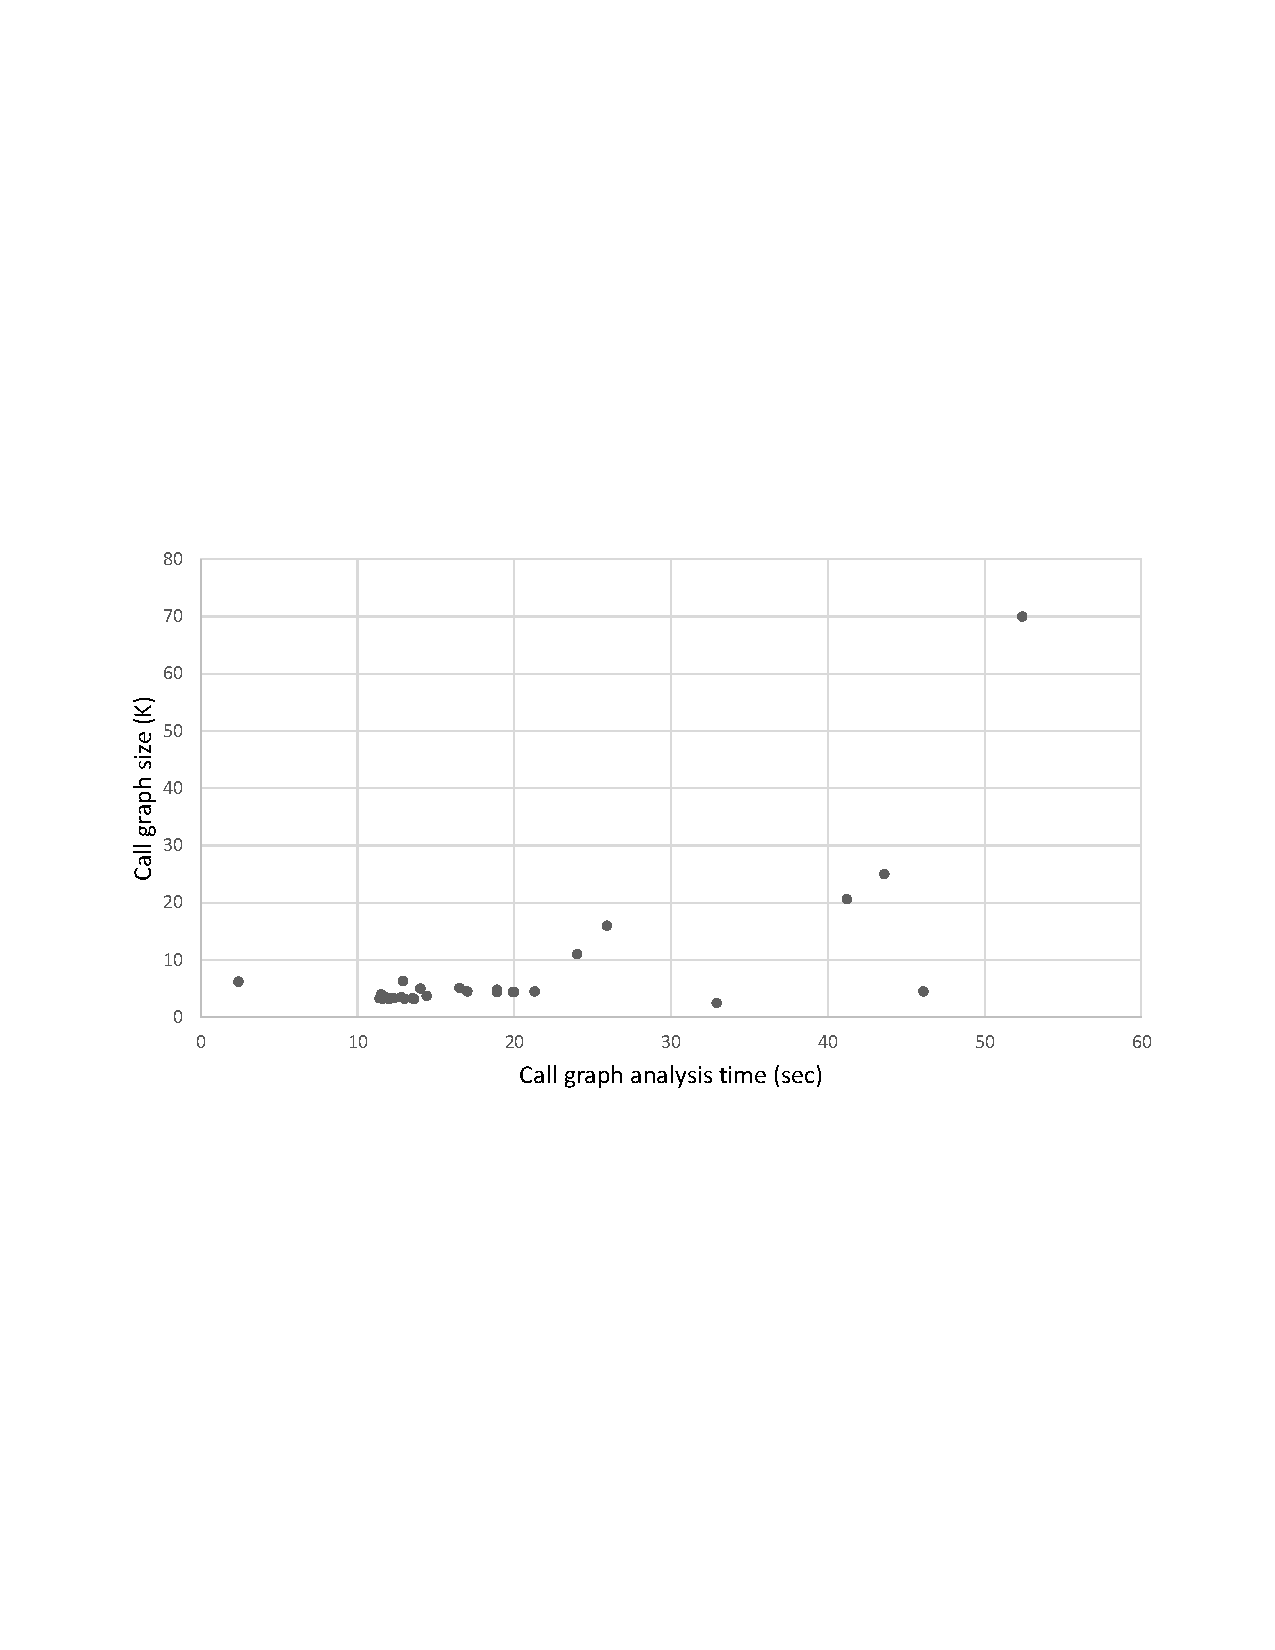
\includegraphics[width=.3\linewidth]{images/CgSizeVsTime.pdf}}
\hfill
&
\subfloat[Variation in static constraint analysis time with number of
constraints.\label{fig:perf:constraints}]
{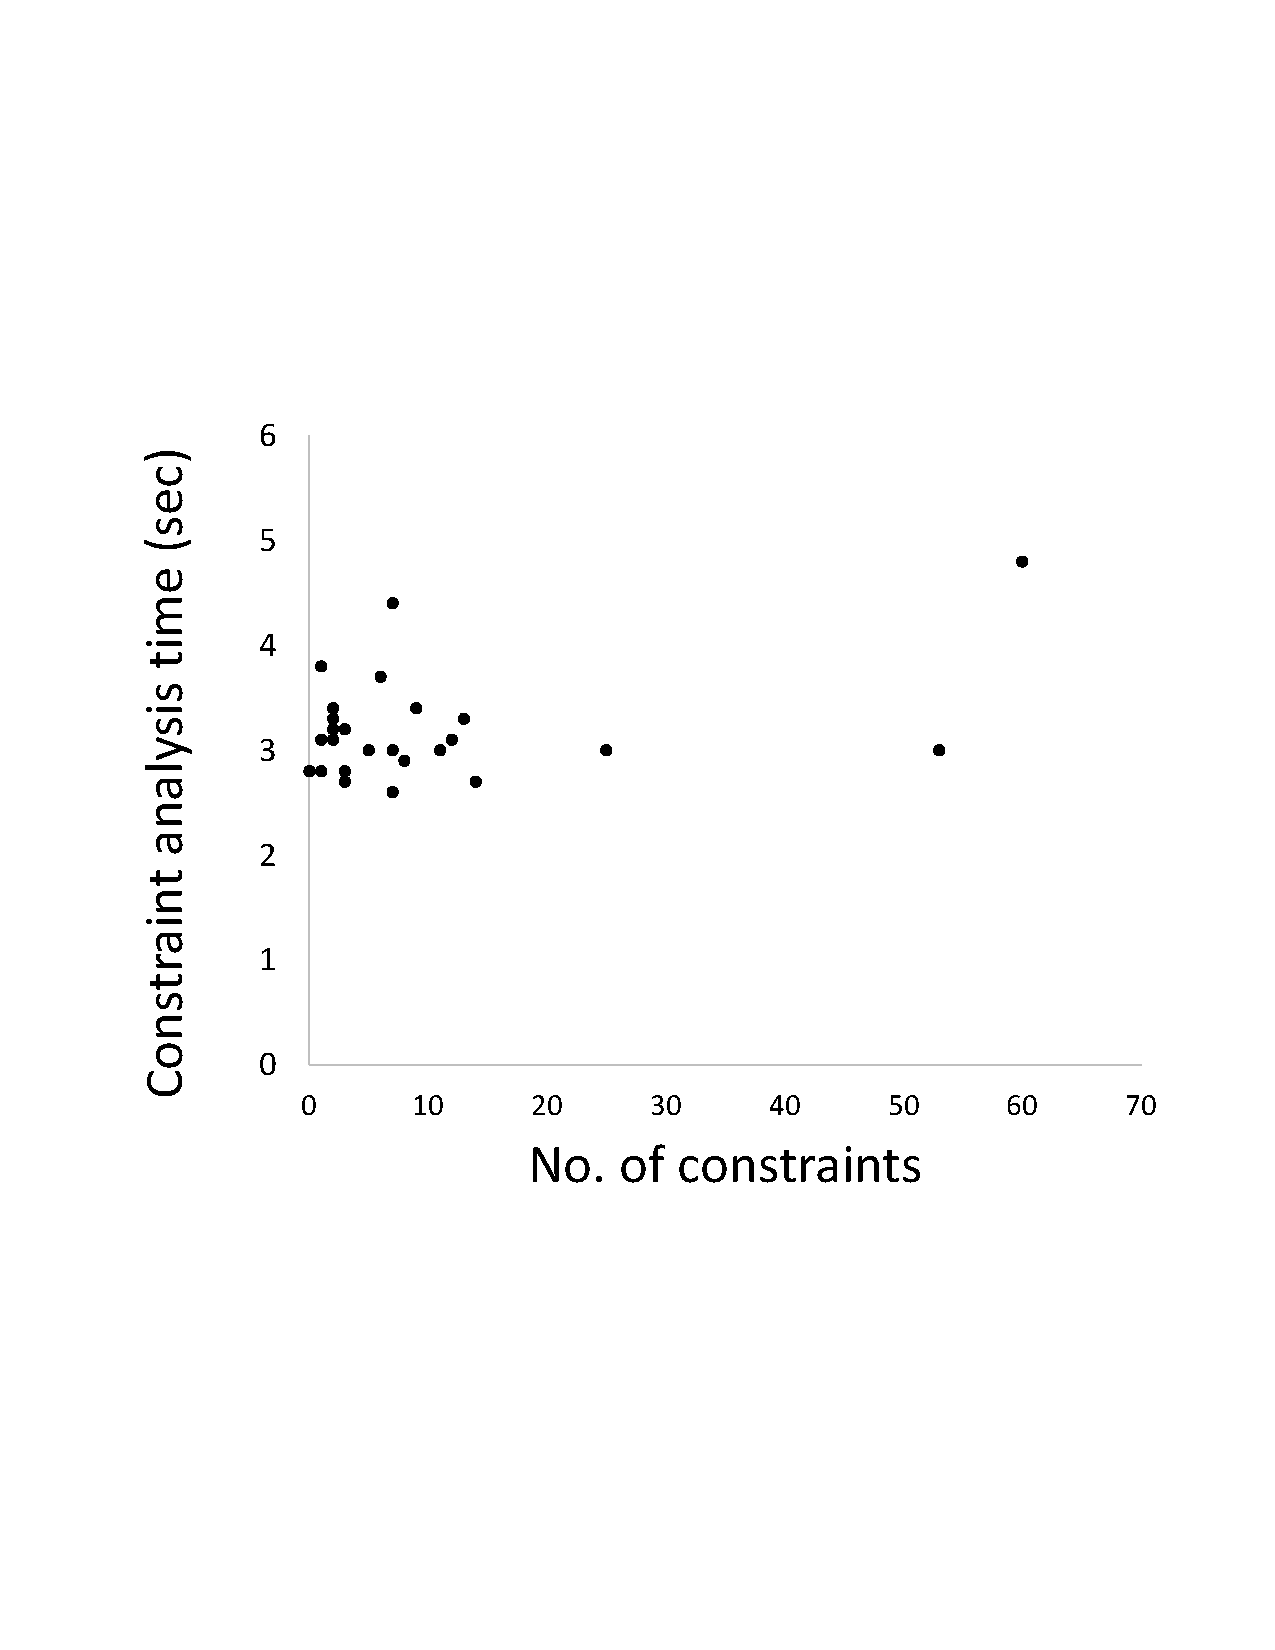
\includegraphics[width=.3\linewidth]{images/ConstraintsVsTime.pdf}
}
\hfill
&
\subfloat[Variation in instrumentation time with \code{Units} to be
instrumented.\label{fig:perf:units}]
{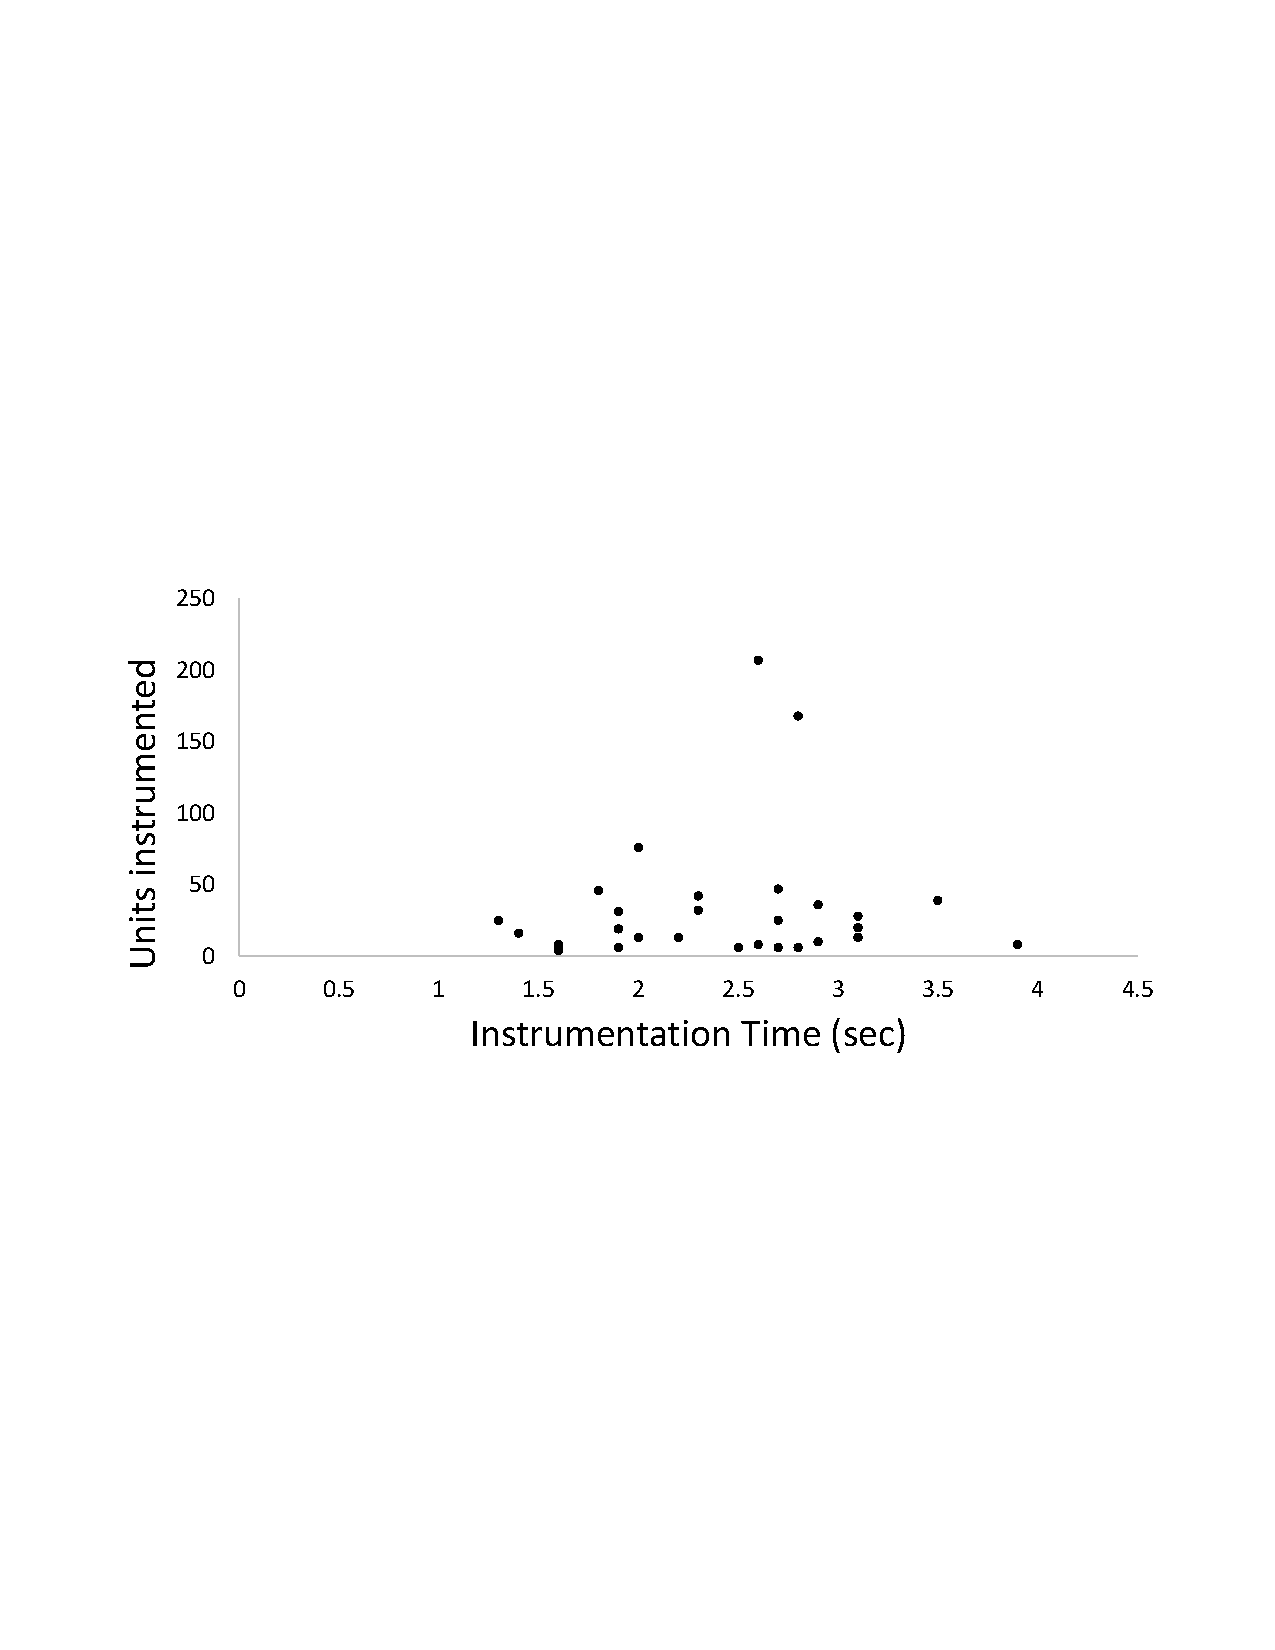
\includegraphics[width=.3\linewidth]{images/InstrumentationVsTime.pdf}}
\hfill
\\
\end{tabular}
\caption{\tool\ evaluation.}
\end{figure*}

\item \textbf{Precision of taint analysis}: \tool\ leverages off-the-shelf
tools (\infoflow) to perform the taint analysis. We measure precision of our
choice of tool by measuring the number of statements in the analyzed code that
are deemed unsafe to patch. Since we could not measure the precision of our
taint analysis on the library benchmarks (as discussed earlier), we select $3$
diverse applications and apply \tool\ in its entirety to obtain a measure of the
precision of the taint analysis. Specifically, for each application we provided
a set of sources, sinks and taint propagators to \infoflow, which listed the
total number of tainted paths, \ie\ paths from a sensitive source to a sink and
thus must not be patched. Table~\ref{tab:taintAnalysis} lists the results. We
observe that the total number of tainted paths is less than $12\%$ across the
applications.

\myparagraph{Threats to validity} Note that \tool\ is dependent on \infoflow\
for achieving precision about the points of instrumentation. However,
\infoflow\ currently has a major limitation---it does not support taint
analysis for multi-threaded programs. Moreover, since it is still under active
development, we observed that when applied to certain applications, \infoflow\
consumed inordinate amounts of memory and crashed. Thus, \tool's precision is
limited by the accuracy of its dependencies. 

\item \textbf{Already handled exceptions}: \tool\ analyzes the call graph to
determine if a potential runtime exception throwing statement is handled higher
up in the call chain or in the same method. In such cases \tool\ must abort the
patching effort considering that the exception is caught with exact exception
type or its base type. This is required else patching will disrupt the normal
control flow of the program.

We measure the extent of this optimization, which prevents disruption of the
control flow using the \textbf{Flow Consistency Index (FCI)} that is calculated
as $FCI = n$, where $n$ is the number of exceptions in the application that
must be ignored \tool\ for forced patching of the bug. Note that $FCI \ge 0$,
and a lower value of $FCI$ is desirable. We observe that patching four bugs
required \tool\ to ignore at most one exception; rest required no changes.

\item \textbf{Cascaded exceptions}: A cascaded exception arises if the
\tool-generated patch creates objects that when used as inputs to other \java\
APIs result in further exceptions.
% patched objects
% are used as a input
% to other methods and violates the specification there.
\tool\ is prone to cascading exceptions because of the limitation of its
intra-procedural analysis and a simple constraint evaluation mechanism. However,
\tool's constraint solver is pluggable and a more sophisticated third party
solvers can easily be integrated.
% This is the limitation
% in our technique in the some complicated cases where it requires develops' 
% attention. The limitation is due to the fact that the analysis for the
% repairing 
% technique is a intra-procedural analysis and the constraint evaluation method is
% very simple. For the constraint evaluation part, the solver is pluggable, we can
% easily replace it with a third party solver.
Specifically, cascaded exceptions may arise if the patch generates \code{String}
objects that represent a malformed string. Further, if we keep the optimization
in \xref{subsubsec:minimizePatchInstrumentation}, then cascaded failures may
occur even for subsequent \code{String} APIs handling the malformed
string following the point of patching. If the optimization is turned
off, \tool\ will automatically patch all relevant \code{String} APIs and thus
handle all cascaded failures involving malformed \code{String} objects.
% 
% Cascaded exception can be noticed
% when the string object we are patching is generation some specific URI or driver
% string which would be used to load or configure something. In such scenario, the
% patch may produce some malformed string. In case there is a cascaded exception 
% in string object, our analysis will take care of it, other wise it would
% abort.

We observe that two benchmarks throw cascaded exceptions even after being
repaired. The cascading was one level deep and triggered exception in another
non-String code (and thus unpatched), which caused the application to crash.

\end{mylist}

Detailed evaluation for each of the bugs in our data set is available at
\url{http://goo.gl/d1zcXD}.

\subsection{Overhead}
\label{sub:overhead}

We measure the overhead of \tool\ across different metrics identified below.

\begin{mylist}

% Apache wicket 100K run patched -> 1090ms, dev fix -> 929 ms
% Eclipse AspectJ weaver 50K run patched -> 8ms, dev fix -> 2 ms
% Apache Tapestry 50K run patched -> 200ms, dev fix -> 178 ms
% Nutch -> 50k run, patched ->183ms, dev patched-> 12 ms
% Hive -> 50k run, patched ->297ms, dev patched-> 99ms

% Constraint analysis dependency : soot invoke + it flashes jimple files.
% 
% Instrumentation dependency : soot overhead for instrumentation  + flashes
% instrumented class files to disk.
% 
% call graph dependency : apart from soot none

 \item \textbf{Execution overhead}: We randomly selected and patched $5$
libraries (Apache Tapestry, Apache Wicket, Eclipse AspectJ Weaver, Hive and
Nutch) from Table~\ref{tab:results} to determine the execution overhead of the
patched class files. We observed that \tool\ reports an average overhead of
$\sim$$2.32\mu$s per call across the $5$ benchmarks for $50K$ runs of the
patched functionality in both the developer's version and \tool's patched
library. The maximum absolute overhead was observed for Hive at $\sim$$3.96\mu$s
per call. The above overhead is imperceptible at human response time scales.

 \item \textbf{Call graph}: The size of the call graph directly governs the time
and memory consumption for \tool. Figure~\ref{fig:perf:callgraph} shows the
results for the benchmarks analyzed from our data set. The overall analysis
time was under a minute for all the benchmarks. We observed that even for a call
graph of $\sim$$70K$ nodes (for \code{Wicket}), \tool\ required just $52.4$s
and $210$MB memory.

 \item \textbf{Constraint set}: \tool\ performs an exhaustive multi-pass
analysis to gather and evaluate the set of constraints for generating patches. A
higher number of constraints and their complexity increases the duration of
\tool's analysis. Figure~\ref{fig:perf:constraints} compares the time required
for static constraint collection and evaluation with an increasing number of
constraints for the benchmarks used in our data set. We observe that across
all the benchmarks used, \tool\ required at most $\sim$$5$s for collecting and
evaluating the constraints.

\item \textbf{Instrumentation overhead}: \tool\ performs bytecode
instrumentation for actual patching. Figure~\ref{fig:perf:units} shows the
variation in instrumentation time with increasing number of \code{Units} to be
patched. We observe that even without optimization discussed in
\xref{subsec:optimizations}, \tool\ takes under $4$s to instrument all
\code{Units} across all benchmarks. We believe that this time would be even
less with the optimizations enabled, which significantly decrease the number of
\code{Units} to be instrumented, and is evident in Table~\ref{tab:results} where
column $\mathcal{IC}_{WO}$ is much less than $\mathcal{IC}_{NO}$.

%  \item \textbf{Number of \code{String} objects}: \tool\ performs exhaustive
% optimizations to limit the static and dynamic instrumentations at points of
% interest. Thus, \tool's performance is also dependent on the number of
% \code{String} objects. Figure~\ref{fig:perf:strings} plots the trend in analysis
% time as a function of the \code{String} objects generated for our benchmarks.
% We observer that \todo{Add details later.}.

\end{mylist}

\subsection{Case studies}
\label{sub:casestudies}

We now report on experiences gained when using \tool\ to patch several of the
bugs reported in Table~\ref{tab:results}.

\begin{mylist}

 \item The bug~\cite{ARIES1204} as reported in the repository for Apache Aries
cited String related issues. However, our investigation showed that the bug was
actually in the ASM framework that was invoked by Aries, and not in the was
actually not in the Aries framework as originally reported. Thus, we patched the
particular ASM methods containing the bugs, and retested it with the Aries
framework to ensure conformance.

 \item The bug in Commons Math~\cite{MATH198} had a bug related to incorrect
formatting of the input string. However, it threw a completely irrelevant
exception (\code{IndexOutOfBound}) instead of the \code{NumberFormatException},
which contains the information of the malformed string. The \tool-generated
patch fixes the undesirable behavior.

 \item The bug in OfBiz~\cite{OFBIZ4237} throws a custom shutdown exception,
when in fact it should throw a \code{StringIndexOutOfBoundsException} due to a
\code{substring} invocation with incorrect bounds. This ultimately causes the
library to throw some high priority exception and ultimately crash if not handed
properly by the application. The patched version of the library catches the
correct exception.

 \item The code to trigger bugs in some libraries, including Apache Commons
Compress, Commons Lang, Commons Math and Ofbiz, each had string operations
wrapped in \code{try-catch} block that were handled by \code{Exception} class,
\ie\ the base type of all exceptions. However, \tool\ checks for already
handled runtime exceptions during its call graph analysis, and thus did not
patch the bugs. We turned off the call graph analysis module to force \tool\ to
generate the relevant patch for the bug.

 \item We also noticed several instances where the developer code does not
follow proper programming practices regarding exception handling. For example,
the SOAP bug~\cite{SOAP130} was reported for a faulty \code{substring} call that
threw a \code{StringIndexOutOfBoundsException}. The entire method was wrapped in
a \code{try-catch} that included the faulty substring call along with other
servlet operations. However, the \code{catch} block handled the generic
\code{Exception}, which is the base class of all exceptions. Thus, both servlet
exceptions or \code{IndexOutOfBoundException} from the \code{substring} call
were handled in a generic fashion. \tool's patched library ensures that
exceptions originating from the \code{substring} call are handled properly.

\end{mylist}


% \begin{figure}[t]
% \centering
% 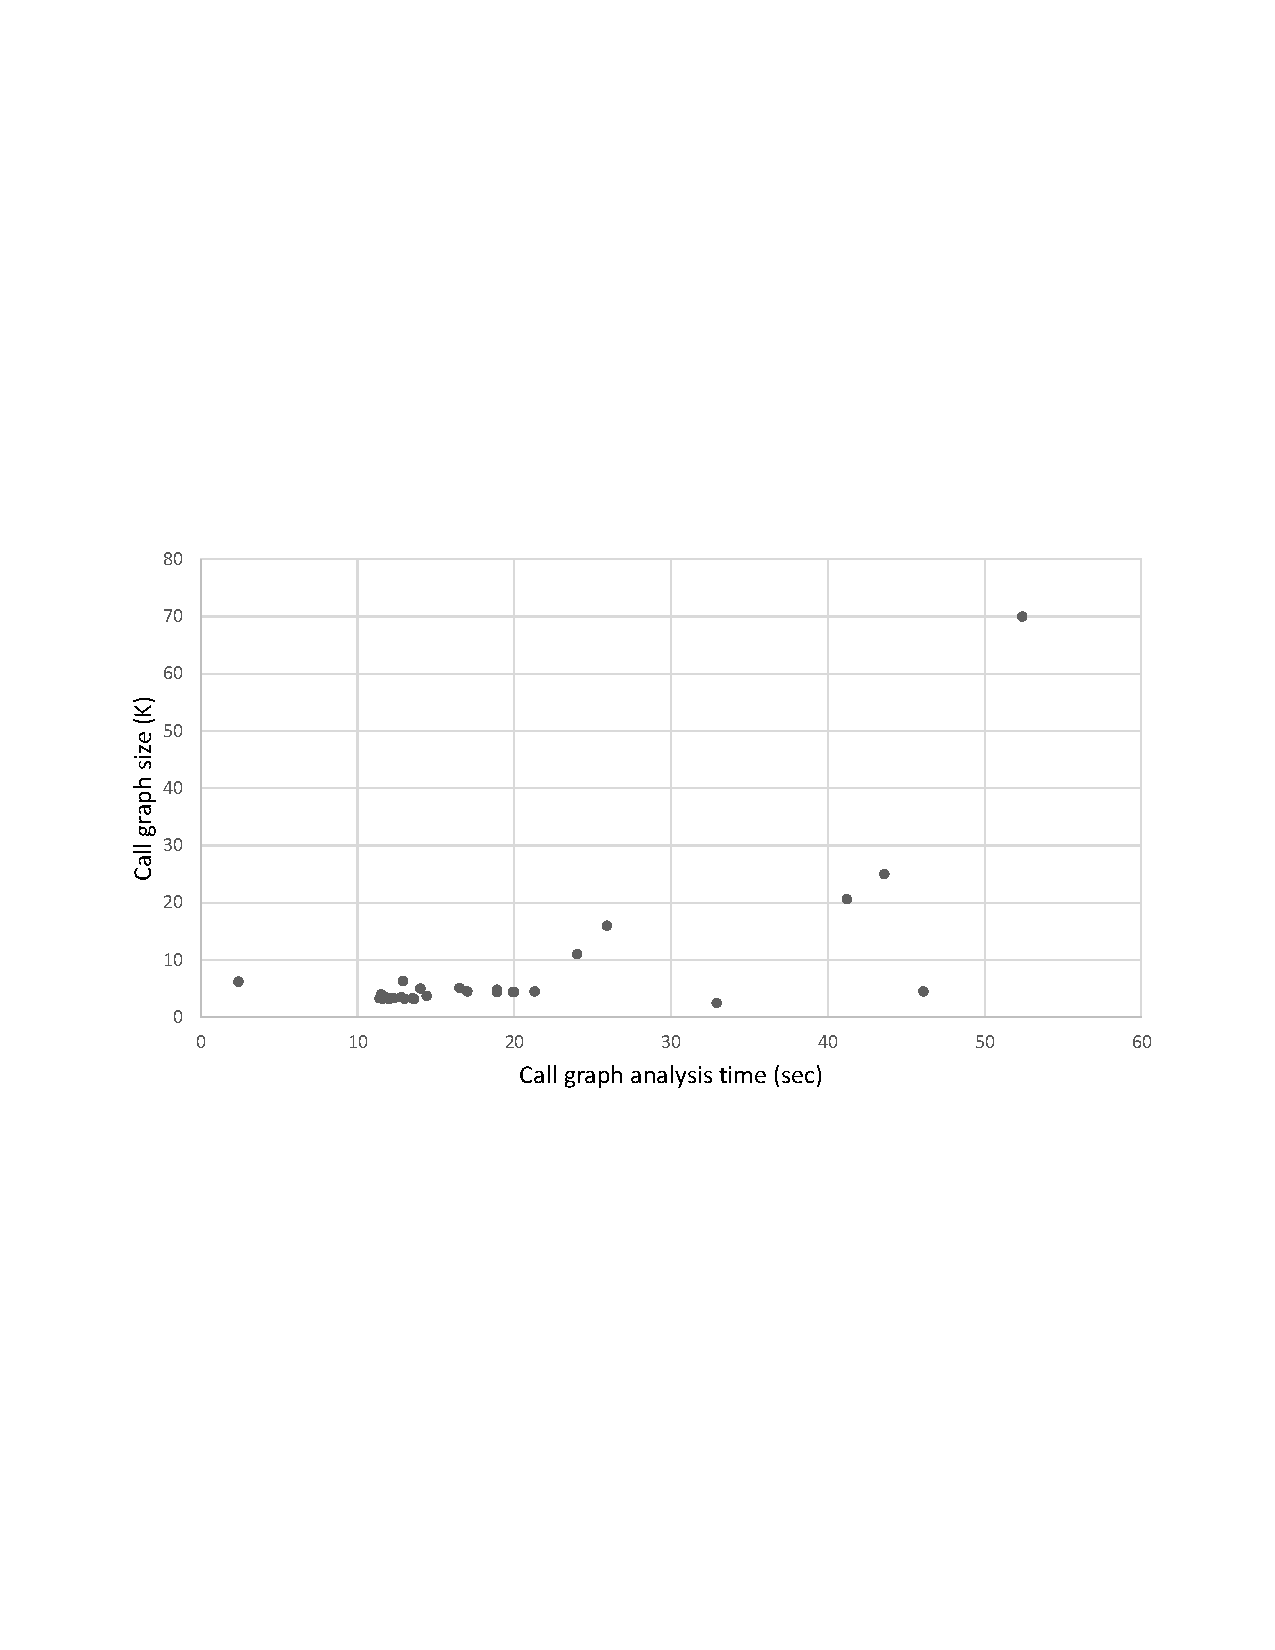
\includegraphics[scale = .45]{images/CgSizeVsTime.pdf}
% \caption{Performance statistics of call graph size vs. time}
% \label{fig:perf:callgraph}
% \end{figure}
% 
% 
% \begin{figure}[t]
% \centering
% 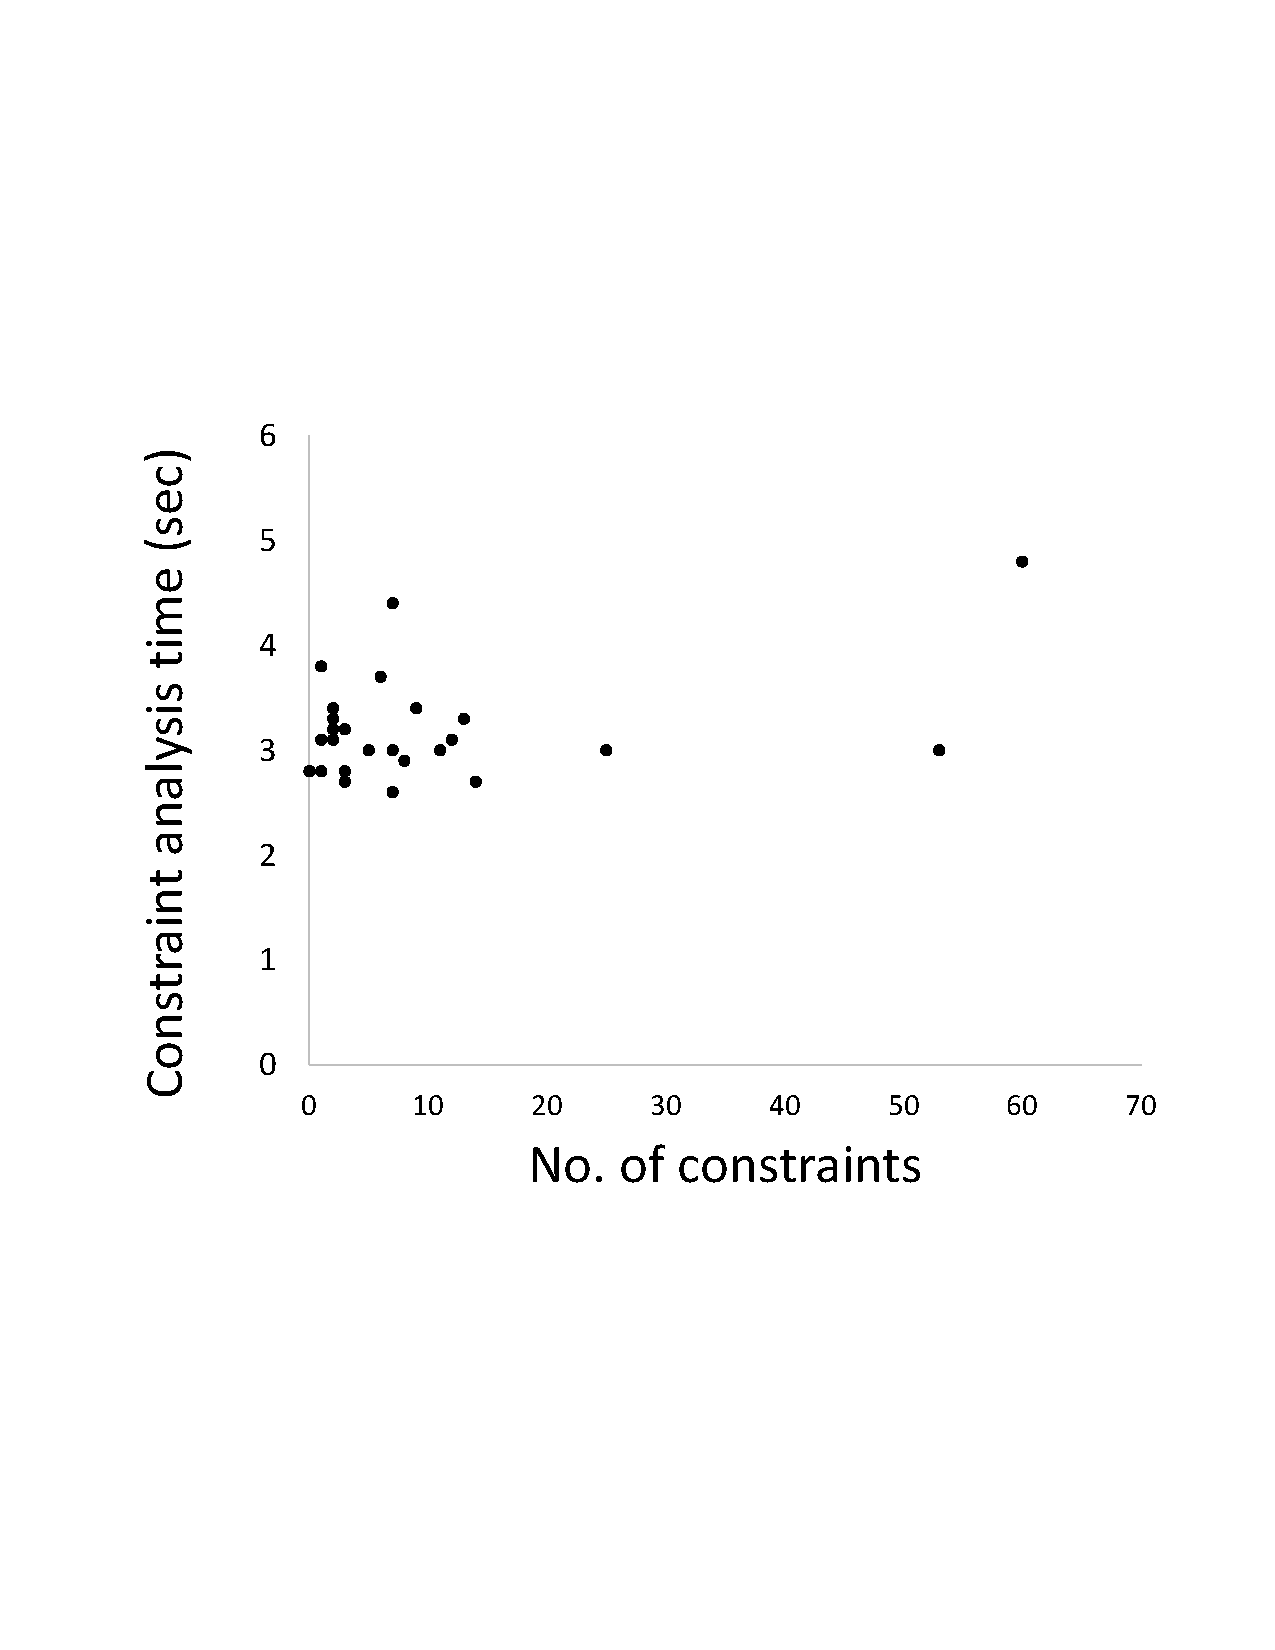
\includegraphics[scale = .31]{images/ConstraintsVsTime.pdf}
% \caption{Performance statistics of constraint vs. time}
% \label{fig:perf:constraints}
% \end{figure}
% 
% \begin{figure}[t]
% \centering
% 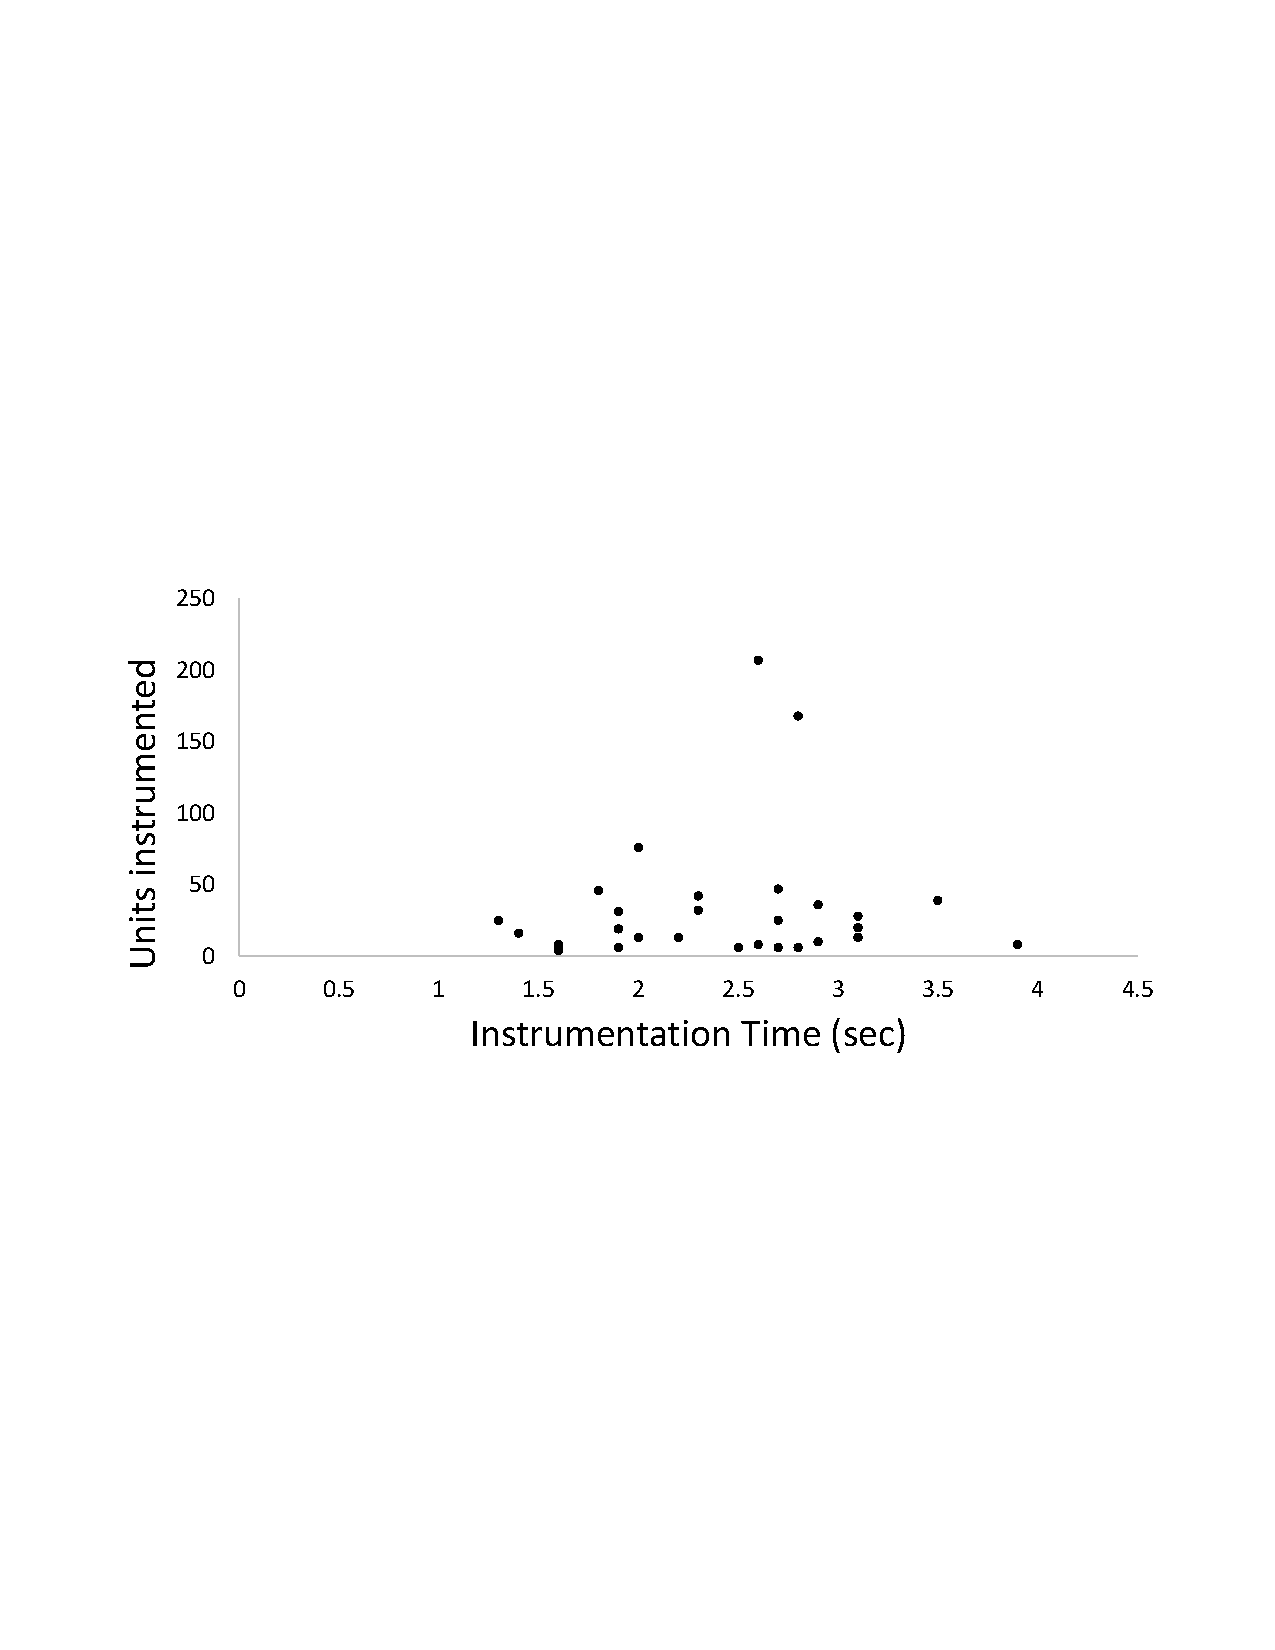
\includegraphics[scale = .48]{images/InstrumentationVsTime.pdf}
% \caption{Performance statistics of instrumentation size vs time}
% \label{fig:constraintHisto}
% \end{figure}


%not required
% \begin{figure}
%         \centering
%         \begin{subfigure}[b]{0.3\textwidth}
%                 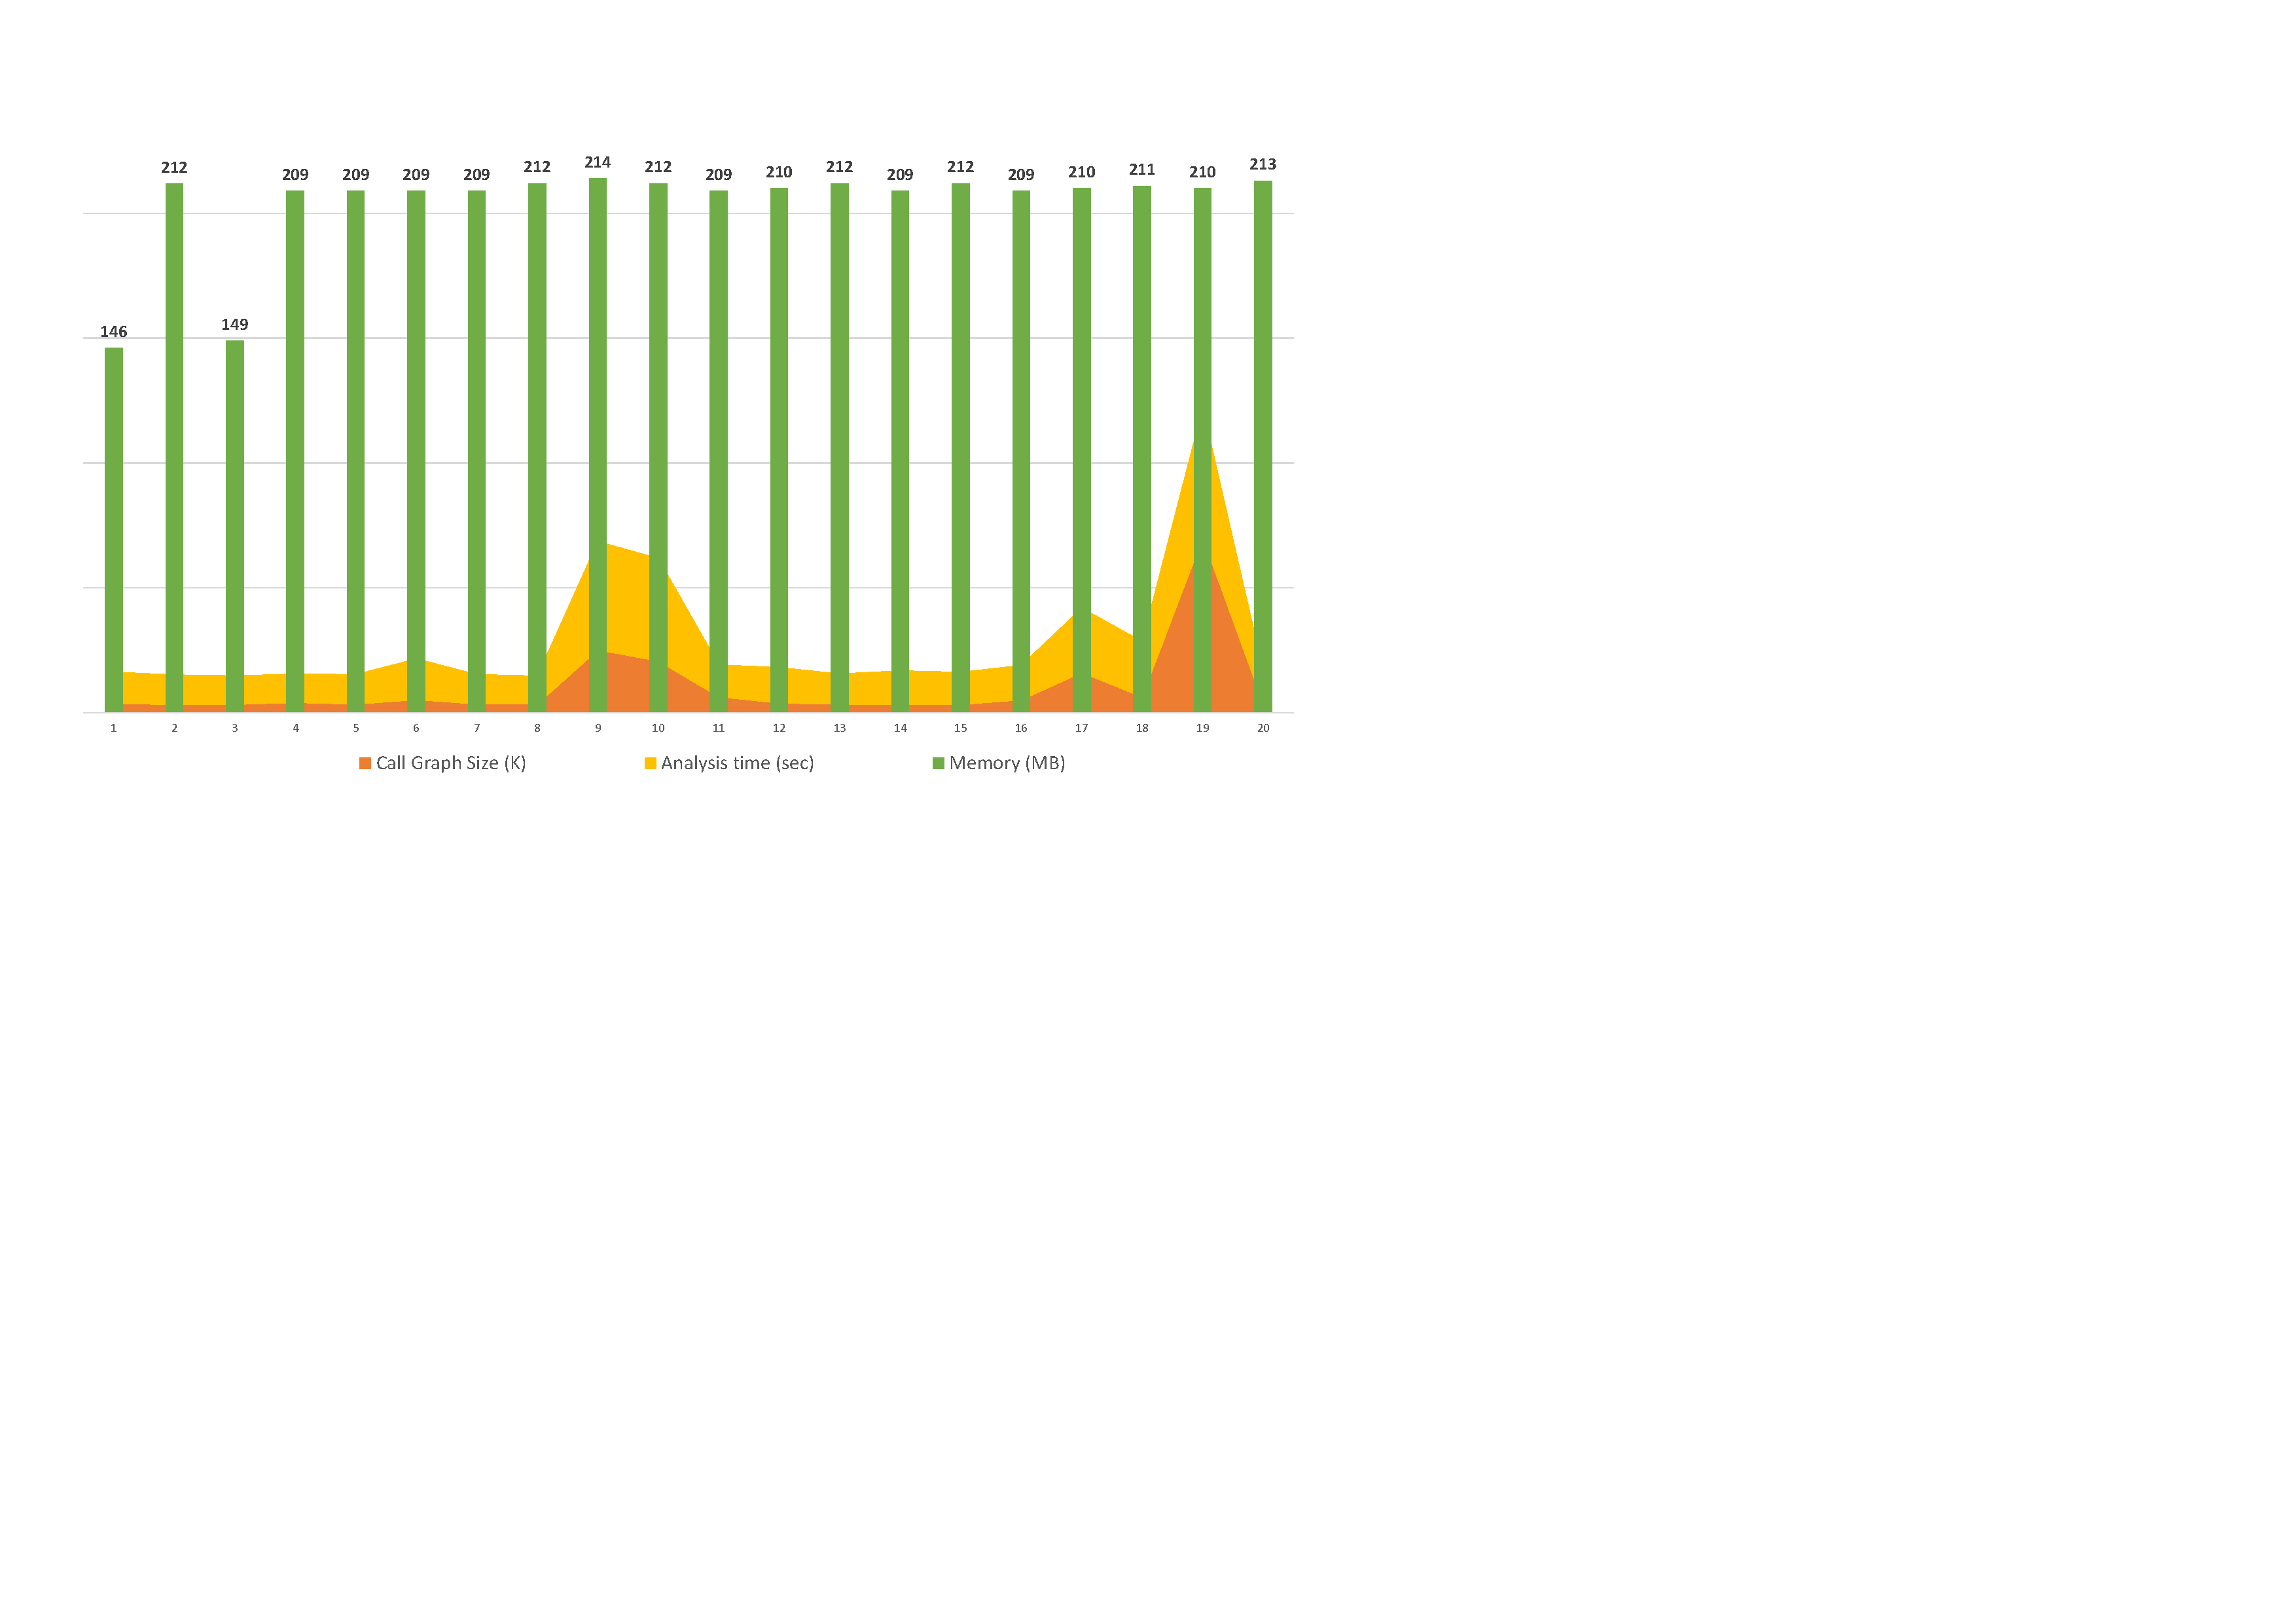
\includegraphics[width=\textwidth]{images/CallGraphHisto.pdf}
%                 \caption{A gull}
%                 \label{fig:gull}
%         \end{subfigure}%
%         ~ %add desired spacing between images, e. g. ~, \quad, \qquad, \hfill etc.
%           %(or a blank line to force the subfigure onto a new line)
%         \begin{subfigure}[b]{0.3\textwidth}
%                 \includegraphics[width=\textwidth]{tiger}
%                 \caption{A tiger}
%                 \label{fig:tiger}
%         \end{subfigure}
%         ~ %add desired spacing between images, e. g. ~, \quad, \qquad, \hfill etc.
%           %(or a blank line to force the subfigure onto a new line)
%         \begin{subfigure}[b]{0.3\textwidth}
%                 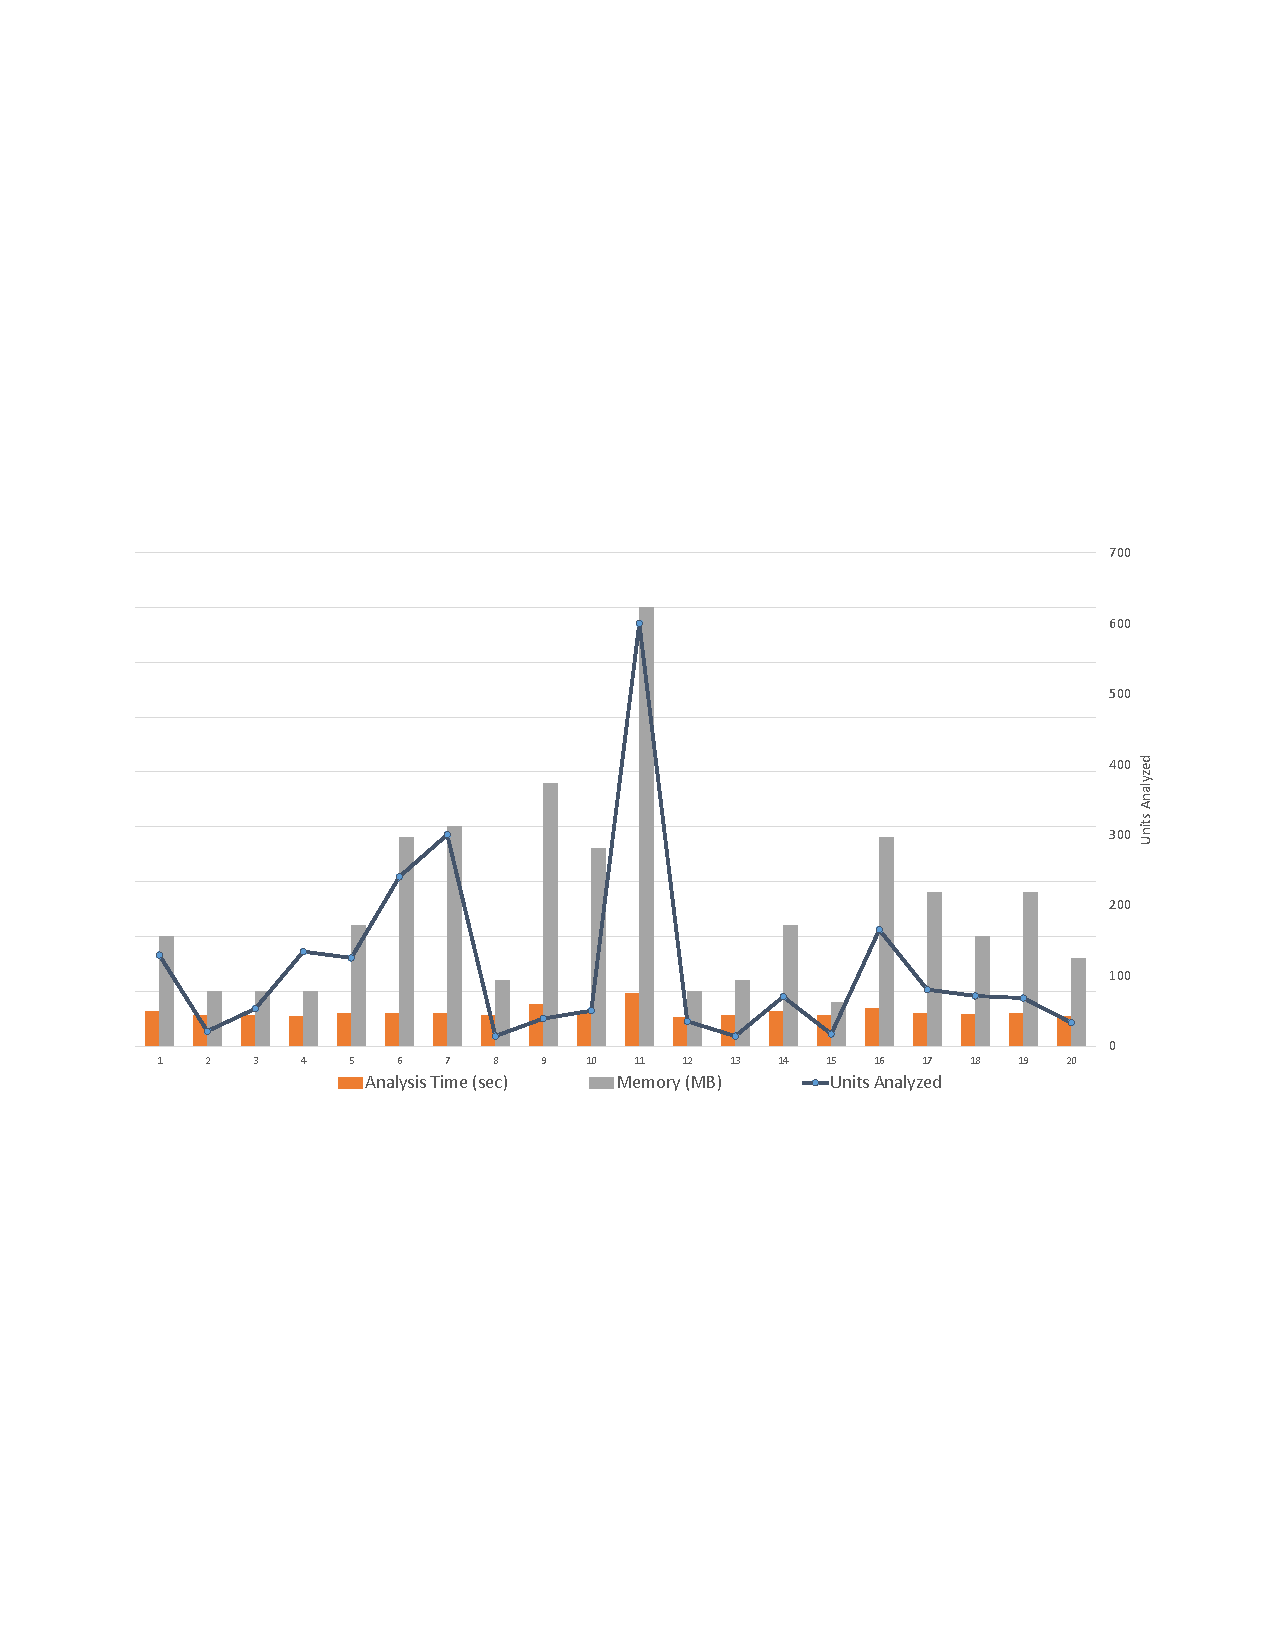
\includegraphics[width=\textwidth]{images/ConstraintHisto.pdf}
%                 \caption{A mouse}
%                 \label{fig:mouse}
%         \end{subfigure}
%         \caption{Pictures of animals}\label{fig:animals}
% \end{figure}
